
\documentclass[10pt]{article}

\usepackage[a4paper,margin=0.65in]{geometry}
\usepackage{amsmath,amssymb}
\usepackage{graphicx}
\usepackage{booktabs}
\usepackage{array}
\usepackage{float}
\usepackage{hyperref}
\usepackage{enumitem}
\usepackage{xcolor}
\usepackage{tikz}
\usetikzlibrary{positioning,arrows.meta,shapes.geometric,fit,calc}

\setlist{nosep,leftmargin=*}
\renewcommand{\arraystretch}{1.2}
\setlength{\parindent}{0pt}
\setlength{\parskip}{2pt}

\tikzset{
layer/.style={
draw,
rounded corners,
minimum width=1.7cm,
minimum height=0.65cm,
align=center,
fill=blue!10,
font=\scriptsize
},
smalllayer/.style={
draw,
rounded corners,
minimum width=1.35cm,
minimum height=0.58cm,
align=center,
fill=green!10,
font=\scriptsize
},
arrow/.style={
-{Latex[length=2mm]},
thin
}
}

\begin{document}

%%%%%%%%%%%%%%%%%%%%%%%%%%%%%%%%%%%%%%%%%%%%%%%%%%%%%%%%%%%%
% TITLE
%%%%%%%%%%%%%%%%%%%%%%%%%%%%%%%%%%%%%%%%%%%%%%%%%%%%%%%%%%%%

\begin{center}

{\large\textbf{Shiv Nadar University Chennai}}

\vspace{2mm}

{\normalsize\textbf{CS3807 -- Deep Learning Laboratory}}

\vspace{2mm}

{\large\textbf{Experiment 6 - Amrut Anand - Roll: 24011101003}}

\vspace{1mm}

{\normalsize\textbf{End-to-End Study of RNN, LSTM and GRU for}}

{\normalsize\textbf{Sequence Learning and Video Understanding}}

\end{center}

\vspace{3mm}

\begin{tabular}{|p{3.4cm}|p{9.0cm}|p{1.4cm}|}
\hline
Degree \& Branch &
B.Tech Artificial Intelligence \& Data Science &
Semester V\\
\hline
Subject Code \& Name &
CS3807 -- Deep Learning Laboratory &
AY: 2026--27\\
\hline
\end{tabular}


%%%%%%%%%%%%%%%%%%%%%%%%%%%%%%%%%%%%%%%%%%%%%%%%%%%%%%%%%%%%
\section*{1. Objective}

The objective of this experiment is to develop an end-to-end understanding of
recurrent sequence learning by implementing and comparing Vanilla RNN, LSTM
and GRU models. The experiment also introduces Backpropagation Through Time
(BPTT), the limitations of conventional RNNs, and the use of CNN-extracted
features with recurrent networks for video understanding.

The experiment uses the UCI Human Activity Recognition Using Smartphones
dataset as the primary sequence dataset. Students will prepare temporal input
sequences, visualize them, train RNN/LSTM/GRU models, compare their
performance, analyze convergence and generalization, and extend the pipeline
to video understanding using CNN feature extraction followed by an LSTM or
GRU.

A small synthetic sequence-to-sequence task is included at the end to
demonstrate the encoder--decoder framework.

%%%%%%%%%%%%%%%%%%%%%%%%%%%%%%%%%%%%%%%%%%%%%%%%%%%%%%%%%%%%
\section*{2. Dataset and Experimental Setup}

\textbf{Primary Dataset: UCI Human Activity Recognition Using Smartphones}

The UCI Human Activity Recognition (HAR) dataset contains smartphone sensor
measurements collected from subjects performing six activities:

\begin{itemize}
\item WALKING
\item WALKING\_UPSTAIRS
\item WALKING\_DOWNSTAIRS
\item SITTING
\item STANDING
\item LAYING
\end{itemize}

The experiment should use the raw inertial signal files rather than only the
already-computed 561-feature vectors. Each activity window contains 128
temporal measurements. The three-axis body acceleration, three-axis
gyroscope and three-axis total acceleration signals provide nine channels.

Thus, the desired input representation is

\[
X\in\mathbb{R}^{N\times128\times9}.
\]

The dataset can be obtained from:

\url{https://archive.ics.uci.edu/dataset/240/human+activity+recognition+using+smartphones}

\textbf{Recommended laboratory subset:} To keep execution time small, use
the first 1500--3000 training windows while preserving all six classes and
approximately balanced class representation. For a complete study, the full
training and test partitions may be used.

\textbf{Important:} The same train/validation/test protocol and preprocessing
must be used for RNN, LSTM and GRU so that the comparison is controlled.

\subsection*{Expected Input}

For one sample:

\[
X_i\in\mathbb{R}^{128\times9}.
\]

For a batch of 32 samples:

\[
X_{\mathrm{batch}}\in\mathbb{R}^{32\times128\times9}.
\]

The dimensions represent:

\begin{center}
\begin{tabular}{|c|c|l|}
\hline
Dimension & Meaning & Example\\
\hline
$N$ & Number of sequences & 1500\\
$T$ & Time steps per sequence & 128\\
$F$ & Features/channels per time step & 9\\
\hline
\end{tabular}
\end{center}

Therefore, the model must receive a three-dimensional tensor rather than a
conventional two-dimensional tabular matrix.

%%%%%%%%%%%%%%%%%%%%%%%%%%%%%%%%%%%%%%%%%%%%%%%%%%%%%%%%%%%%
\section*{3. Overall Experimental Pipeline}

The complete sequence-classification pipeline is:

\begin{center}
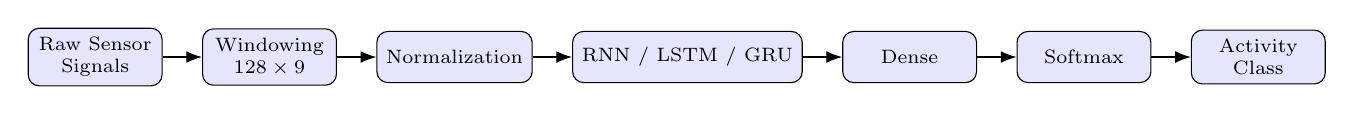
\begin{tikzpicture}[node distance=5mm]
\node[layer](a){Raw Sensor\\Signals};
\node[layer,right=of a](b){Windowing\\$128\times9$};
\node[layer,right=of b](c){Normalization};
\node[layer,right=of c](d){RNN / LSTM / GRU};
\node[layer,right=of d](e){Dense};
\node[layer,right=of e](f){Softmax};
\node[layer,right=of f](g){Activity\\Class};

\foreach \x/\y in {a/b,b/c,c/d,d/e,e/f,f/g}
\draw[arrow](\x)--(\y);
\end{tikzpicture}
\end{center}

The three recurrent models must use the same input, output layer, optimizer,
batch size and evaluation protocol.

%%%%%%%%%%%%%%%%%%%%%%%%%%%%%%%%%%%%%%%%%%%%%%%%%%%%%%%%%%%%
\section*{4. Preprocessing}

Perform the following preprocessing steps:

\begin{enumerate}
\item Load the raw inertial signals.
\item Arrange every observation window as $128\times9$.
\item Assign one activity label to each window.
\item Encode the six activity labels.
\item Normalize the input using statistics calculated from the training data.
\item Create training, validation and test sets.
\item Verify the class distribution.
\end{enumerate}

\textbf{Suggested split:}

\[
70\% \text{ training},\qquad
15\% \text{ validation},\qquad
15\% \text{ testing}.
\]

The test data must not be used during model selection or hyperparameter tuning.

\subsection*{Expected Preprocessing Output}
\begin{verbatim}
Input tensor shape:
Training   : (2100, 128, 9)
Validation : (450, 128, 9)
Testing    : (2947, 128, 9)
Number of classes: 6
Number of features per time step: 9
Sequence length: 128
\end{verbatim}
\section*{5. Temporal Data Visualization}

Select representative sequences from at least three different activity
classes.

\textbf{Plot 1: Sensor signal versus time}

\begin{itemize}
\item X-axis: Time step (1--128)
\item Y-axis: Sensor value
\item Plot at least three representative channels.
\item Include examples from different activity classes.
\end{itemize}

Students should observe that temporal patterns differ across activities.

\textbf{Required inference:}

\begin{enumerate}
\item What temporal pattern is visible?
\item Which activities exhibit similar patterns?
\item Why is the ordering of measurements important?
\end{enumerate}

%%%%%%%%%%%%%%%%%%%%%%%%%%%%%%%%%%%%%%%%%%%%%%%%%%%%%%%%%%%%
\section*{6. Vanilla RNN Architecture}

A Vanilla RNN maintains a hidden state that is updated at every time step:

\[
h_t=\tanh(W_xx_t+W_hh_{t-1}+b_h).
\]

The output can be written as

\[
y_t=g(W_yh_t+b_y).
\]

For sequence classification, the final hidden representation can be passed
to a classifier.

\begin{center}
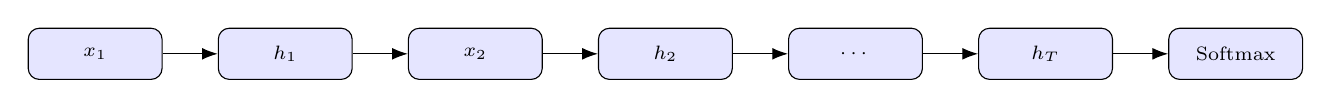
\begin{tikzpicture}[node distance=7mm]
\node[layer](x1){$x_1$};
\node[layer,right=of x1](h1){$h_1$};
\node[layer,right=of h1](x2){$x_2$};
\node[layer,right=of x2](h2){$h_2$};
\node[layer,right=of h2](x3){$\cdots$};
\node[layer,right=of x3](h3){$h_T$};
\node[layer,right=of h3](y){Softmax};

\draw[arrow](x1)--(h1);
\draw[arrow](h1)--(x2);
\draw[arrow](x2)--(h2);
\draw[arrow](h2)--(x3);
\draw[arrow](x3)--(h3);
\draw[arrow](h3)--(y);
\end{tikzpicture}
\end{center}

The diagram represents the unrolled view of an RNN. The same recurrent weights
are reused across time steps.

%%%%%%%%%%%%%%%%%%%%%%%%%%%%%%%%%%%%%%%%%%%%%%%%%%%%%%%%%%%%
\section*{7. Backpropagation Through Time}

When an RNN is unrolled, the loss depends on the sequence of hidden states.
Backpropagation Through Time (BPTT) propagates the error backward through
the recurrent steps.

\begin{center}
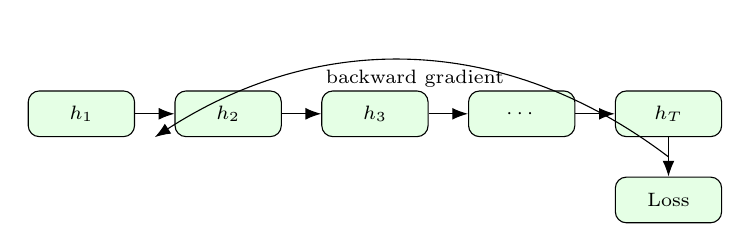
\begin{tikzpicture}[node distance=5mm]
\node[smalllayer](a){$h_1$};
\node[smalllayer,right=of a](b){$h_2$};
\node[smalllayer,right=of b](c){$h_3$};
\node[smalllayer,right=of c](d){$\cdots$};
\node[smalllayer,right=of d](e){$h_T$};
\node[smalllayer,below=of e](l){Loss};

\draw[arrow](a)--(b);
\draw[arrow](b)--(c);
\draw[arrow](c)--(d);
\draw[arrow](d)--(e);
\draw[arrow](e)--(l);

\draw[arrow]($(e.south)!0.5!(l.north)$) to[bend right=35]
node[below,font=\scriptsize]{backward gradient} ($(a.south)!0.5!(b.south)$);
\end{tikzpicture}
\end{center}

Students should explain that repeated multiplication of derivatives through
many time steps can cause gradients to become extremely small or extremely
large.

\subsection*{Challenges}

\begin{itemize}
\item Vanishing gradients
\item Exploding gradients
\item Difficulty learning long-term dependencies
\item Sequential computation and limited parallelism
\end{itemize}

The vanishing-gradient problem can be conceptually represented as

\[
\left|\frac{\partial h_t}{\partial h_{t-k}}\right|\rightarrow0
\]

while exploding gradients correspond to very large gradient magnitudes.

\subsection*{Numerical Exercise}
Given $x_1 = 0.5, x_2 = 0.7, x_3 = 0.2$ and $h_0 = 0, W_x = 0.5, W_h = 0.8, b = 0.1$:
\begin{align*}
h_1 &= \tanh(W_x x_1 + W_h h_0 + b) = \tanh(0.5(0.5) + 0.8(0) + 0.1) = \tanh(0.35) = 0.3364 \\
h_2 &= \tanh(W_x x_2 + W_h h_1 + b) = \tanh(0.5(0.7) + 0.8(0.3364) + 0.1) = \tanh(0.7191) = 0.6164 \\
h_3 &= \tanh(W_x x_3 + W_h h_2 + b) = \tanh(0.5(0.2) + 0.8(0.6164) + 0.1) = \tanh(0.6931) = 0.6000
\end{align*}
\section*{8. RNN Implementation}

Use a small recurrent architecture:

\begin{center}
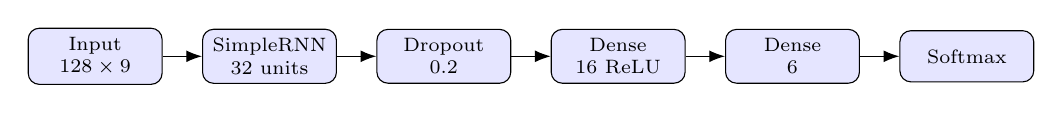
\begin{tikzpicture}[node distance=5mm]
\node[layer](a){Input\\$128\times9$};
\node[layer,right=of a](b){SimpleRNN\\32 units};
\node[layer,right=of b](c){Dropout\\0.2};
\node[layer,right=of c](d){Dense\\16 ReLU};
\node[layer,right=of d](e){Dense\\6};
\node[layer,right=of e](f){Softmax};

\foreach \x/\y in {a/b,b/c,c/d,d/e,e/f}
\draw[arrow](\x)--(\y);
\end{tikzpicture}
\end{center}

\textbf{Suggested training configuration:}

\begin{center}
\begin{tabular}{|l|l|}
\hline
Parameter & Value\\
\hline
Recurrent units & 32\\
Dropout & 0.2\\
Optimizer & Adam\\
Learning rate & $10^{-3}$\\
Batch size & 32\\
Epochs & 30\\
Loss & Sparse categorical cross-entropy\\
\hline
\end{tabular}
\end{center}

%%%%%%%%%%%%%%%%%%%%%%%%%%%%%%%%%%%%%%%%%%%%%%%%%%%%%%%%%%%%
\section*{9. LSTM Architecture}

LSTM introduces a memory cell and gates to control information flow.

The forget gate is

\[
f_t=\sigma(W_f[h_{t-1},x_t]+b_f),
\]

the input gate is

\[
i_t=\sigma(W_i[h_{t-1},x_t]+b_i),
\]

and the output gate is

\[
o_t=\sigma(W_o[h_{t-1},x_t]+b_o).
\]

The candidate cell state is

\[
\tilde{C}_t=
\tanh(W_C[h_{t-1},x_t]+b_C),
\]

and the cell state is

\[
C_t=f_tC_{t-1}+i_t\tilde{C}_t.
\]

The hidden state is

\[
h_t=o_t\tanh(C_t).
\]

\begin{center}
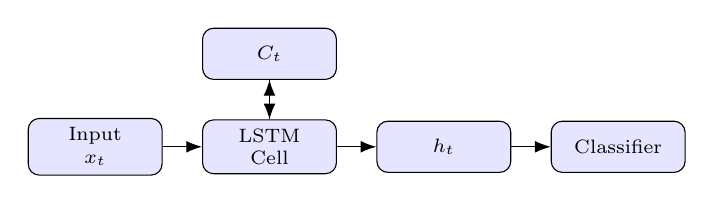
\begin{tikzpicture}[node distance=5mm]
\node[layer](a){Input\\$x_t$};
\node[layer,right=of a](b){LSTM\\Cell};
\node[layer,right=of b](c){$h_t$};
\node[layer,above=of b](d){$C_t$};
\node[layer,right=of c](e){Classifier};

\draw[arrow](a)--(b);
\draw[arrow](b)--(c);
\draw[arrow](b)--(d);
\draw[arrow](c)--(e);
\draw[arrow](d)--(b);
\end{tikzpicture}
\end{center}

\textbf{Required inference:} Explain how the cell state and gates help the
network retain or discard information over long sequences.

%%%%%%%%%%%%%%%%%%%%%%%%%%%%%%%%%%%%%%%%%%%%%%%%%%%%%%%%%%%%
\section*{10. GRU Architecture}

GRU uses two principal gates:

\[
z_t=\sigma(W_z[h_{t-1},x_t]+b_z)
\]

and

\[
r_t=\sigma(W_r[h_{t-1},x_t]+b_r).
\]

The candidate hidden state is

\[
\tilde{h}_t=
\tanh(W_h[r_t\odot h_{t-1},x_t]+b_h).
\]

The hidden state is updated using

\[
h_t=(1-z_t)h_{t-1}+z_t\tilde{h}_t.
\]

\begin{center}
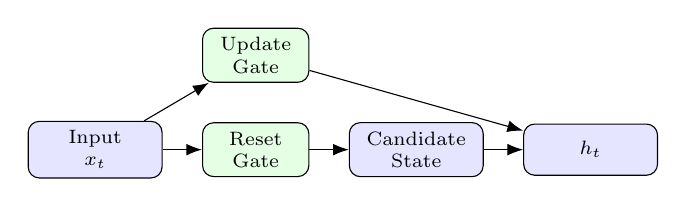
\begin{tikzpicture}[node distance=5mm]
\node[layer](a){Input\\$x_t$};
\node[smalllayer,right=of a](b){Reset\\Gate};
\node[smalllayer,above=of b](c){Update\\Gate};
\node[layer,right=of b](d){Candidate\\State};
\node[layer,right=of d](e){$h_t$};

\draw[arrow](a)--(b);
\draw[arrow](a)--(c);
\draw[arrow](b)--(d);
\draw[arrow](c)--(e);
\draw[arrow](d)--(e);
\end{tikzpicture}
\end{center}

Students should compare the number of gates and state representations in
RNN, LSTM and GRU.

%%%%%%%%%%%%%%%%%%%%%%%%%%%%%%%%%%%%%%%%%%%%%%%%%%%%%%%%%%%%
\section*{11. LSTM and GRU Implementation}

Implement the same classifier used for the RNN, replacing only the recurrent
layer.

\begin{center}
\begin{tabular}{|l|c|c|c|}
\hline
Model & Recurrent Layer & Units & Output Classes\\
\hline
RNN & SimpleRNN & 32 & 6\\
LSTM & LSTM & 32 & 6\\
GRU & GRU & 32 & 6\\
\hline
\end{tabular}
\end{center}

All other experimental conditions should remain unchanged.

%%%%%%%%%%%%%%%%%%%%%%%%%%%%%%%%%%%%%%%%%%%%%%%%%%%%%%%%%%%%
\section*{12. Source Code}
GitHub repository: \href{https://github.com/the-future-codemaster/dl_lab/tree/main/Experiment_6}{https://github.com/the-future-codemaster/dl_lab/tree/main/Experiment_6}

\section*{13. Experimental Outcomes}

\subsection*{Performance Evaluation (Sequence Classification)}
\begin{table}[H]
    \centering
    \begin{tabular}{|c|c|c|c|c|c|c|}
        \hline
        \textbf{Model} & \textbf{Accuracy (\%)} & \textbf{Precision (\%)} & \textbf{Recall (\%)} & \textbf{F1 (\%)} & \textbf{Parameters} & \textbf{Time (s)} \\ \hline
        RNN & 75.60 & 76.06 & 75.02 & 74.78 & 1,974 & 14.58 \\ \hline
        LSTM & 88.80 & 88.85 & 88.94 & 88.83 & 6,006 & 31.85 \\ \hline
        GRU & 88.60 & 88.59 & 88.61 & 88.49 & 4,758 & 39.43 \\ \hline
    \end{tabular}
\end{table}

\subsection*{RNN vs. LSTM vs. GRU Comparison}
\begin{table}[H]
    \centering
    \begin{tabular}{|l|c|c|c|}
        \hline
        \textbf{Property} & \textbf{RNN} & \textbf{LSTM} & \textbf{GRU} \\ \hline
        Hidden state & Yes & Yes & Yes \\ \hline
        Cell state & No & Yes & No \\ \hline
        Forget gate & No & Yes & No \\ \hline
        Input gate & No & Yes & No \\ \hline
        Output gate & No & Yes & No \\ \hline
        Update gate & No & No & Yes \\ \hline
        Reset gate & No & No & Yes \\ \hline
        Parameters & 1,974 & 6,006 & 4,758 \\ \hline
        Training time (s) & 14.58 & 31.85 & 39.43 \\ \hline
        Test F1-score (\%) & 74.78 & 88.83 & 88.49 \\ \hline
    \end{tabular}
\end{table}

\subsection*{Effect of Sequence Length}
\begin{table}[H]
    \centering
    \begin{tabular}{|c|c|c|c|}
        \hline
        \textbf{Sequence Length} & \textbf{RNN F1 (\%)} & \textbf{LSTM F1 (\%)} & \textbf{GRU F1 (\%)} \\ \hline
        32 & 69.68 & 86.67 & 84.55 \\ \hline
        64 & 68.97 & 88.33 & 84.69 \\ \hline
        128 & 69.75 & 87.53 & 88.04 \\ \hline
    \end{tabular}
\end{table}

\subsection*{CNN Feature Extraction (Video Understanding)}
\begin{verbatim}
CNN feature dimension: 1280
Resulting tensor shape supplied to recurrent network: (15, 10, 1280)
\end{verbatim}

\subsection*{Observed Sequence-to-Sequence Output}
\begin{table}[H]
    \centering
    \begin{tabular}{|c|c|c|c|c|}
        \hline
        \textbf{Sample} & \textbf{Input Sequence} & \textbf{Expected Output} & \textbf{Predicted Output} & \textbf{Correct} \\ \hline
        1 & [9, 5, 3, 3] & [3, 3, 5, 9] & [3, 3, 5, 9] & Yes \\ \hline
        2 & [4, 2, 3, 4] & [4, 3, 2, 4] & [4, 3, 2, 2] & No \\ \hline
        3 & [4, 5, 2, 4] & [4, 2, 5, 4] & [4, 2, 5, 2] & No \\ \hline
        4 & [2, 8, 9, 9] & [9, 9, 8, 2] & [9, 9, 8, 2] & Yes \\ \hline
        5 & [7, 5, 7, 2] & [2, 7, 5, 7] & [2, 7, 5, 7] & Yes \\ \hline
    \end{tabular}
\end{table}

\subsection*{Sequence-to-Sequence Evaluation}
\begin{verbatim}
Token Accuracy: 92.50%
Sequence Accuracy: 70.00%
Final training loss: 0.0929
Final validation loss: 0.0924
\end{verbatim}

\section*{14. Plots and Inferences}

\subsection*{Plot 1: Sensor Signal vs. Time}
\begin{figure}[H]
    \centering
    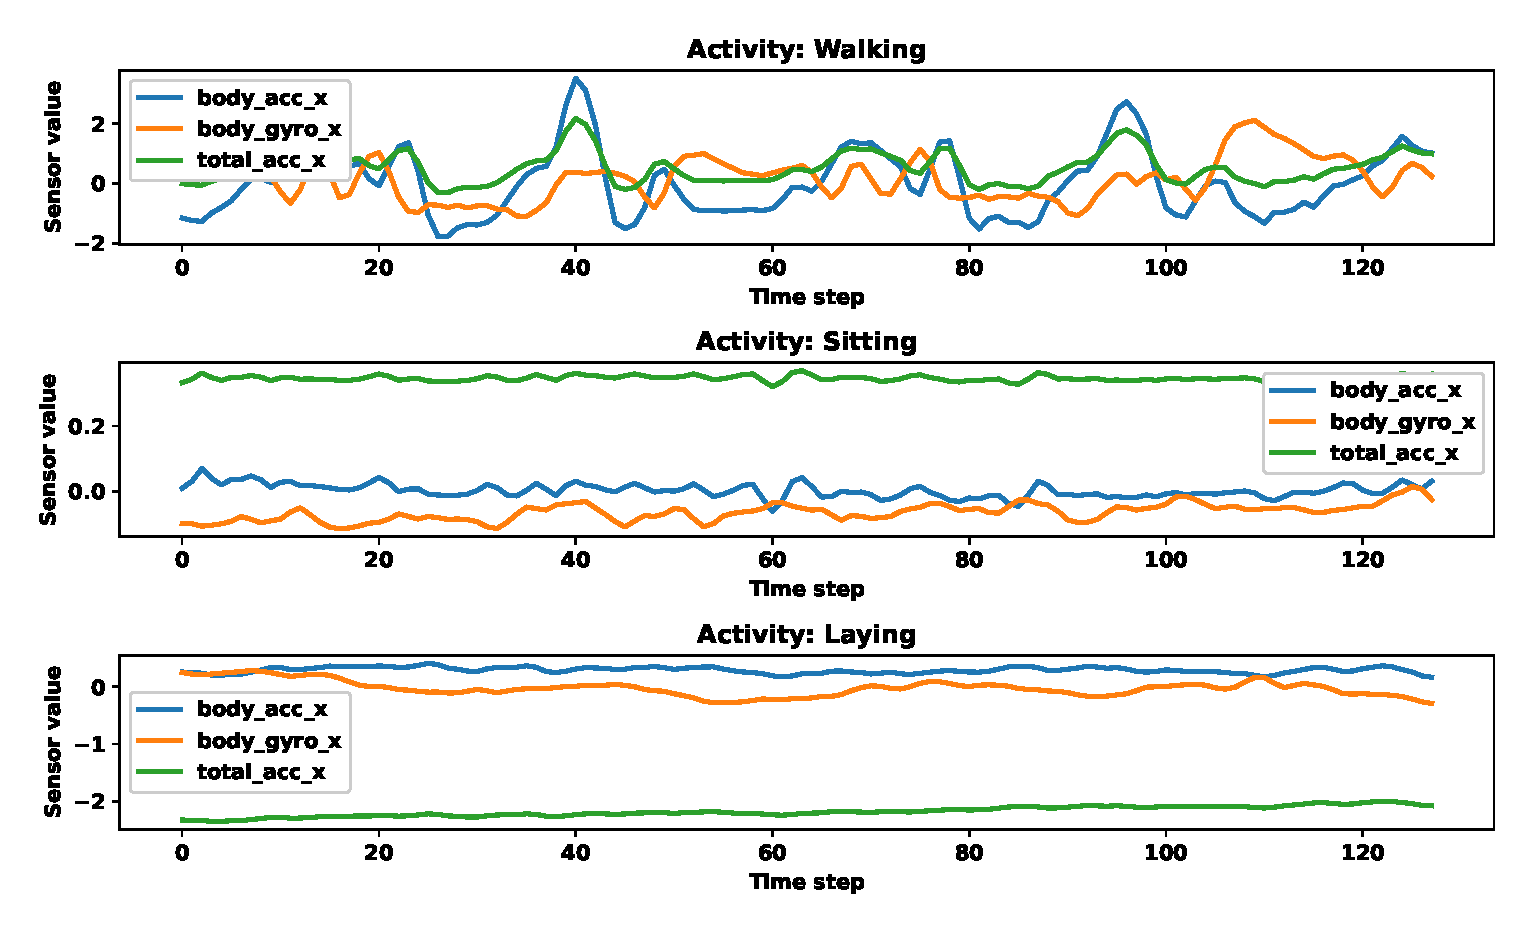
\includegraphics[width=\textwidth]{Plot1_SensorSignals.eps}
\end{figure}
\textbf{Interpretation:} This plot compares the normalized sensor readings across three distinct activities. Active tasks, such as Walking, exhibit high-variance periodic oscillations caused by repetitive foot-strikes. Meanwhile, static tasks like Sitting show flat, constant values that reflect only gravitational offsets. This demonstrates that the time-series order is critical; shuffling the measurements would completely destroy the periodic gait patterns needed to accurately classify dynamic activities.

\subsection*{Plot 2: Training and Validation Loss}
\begin{figure}[H]
    \centering
    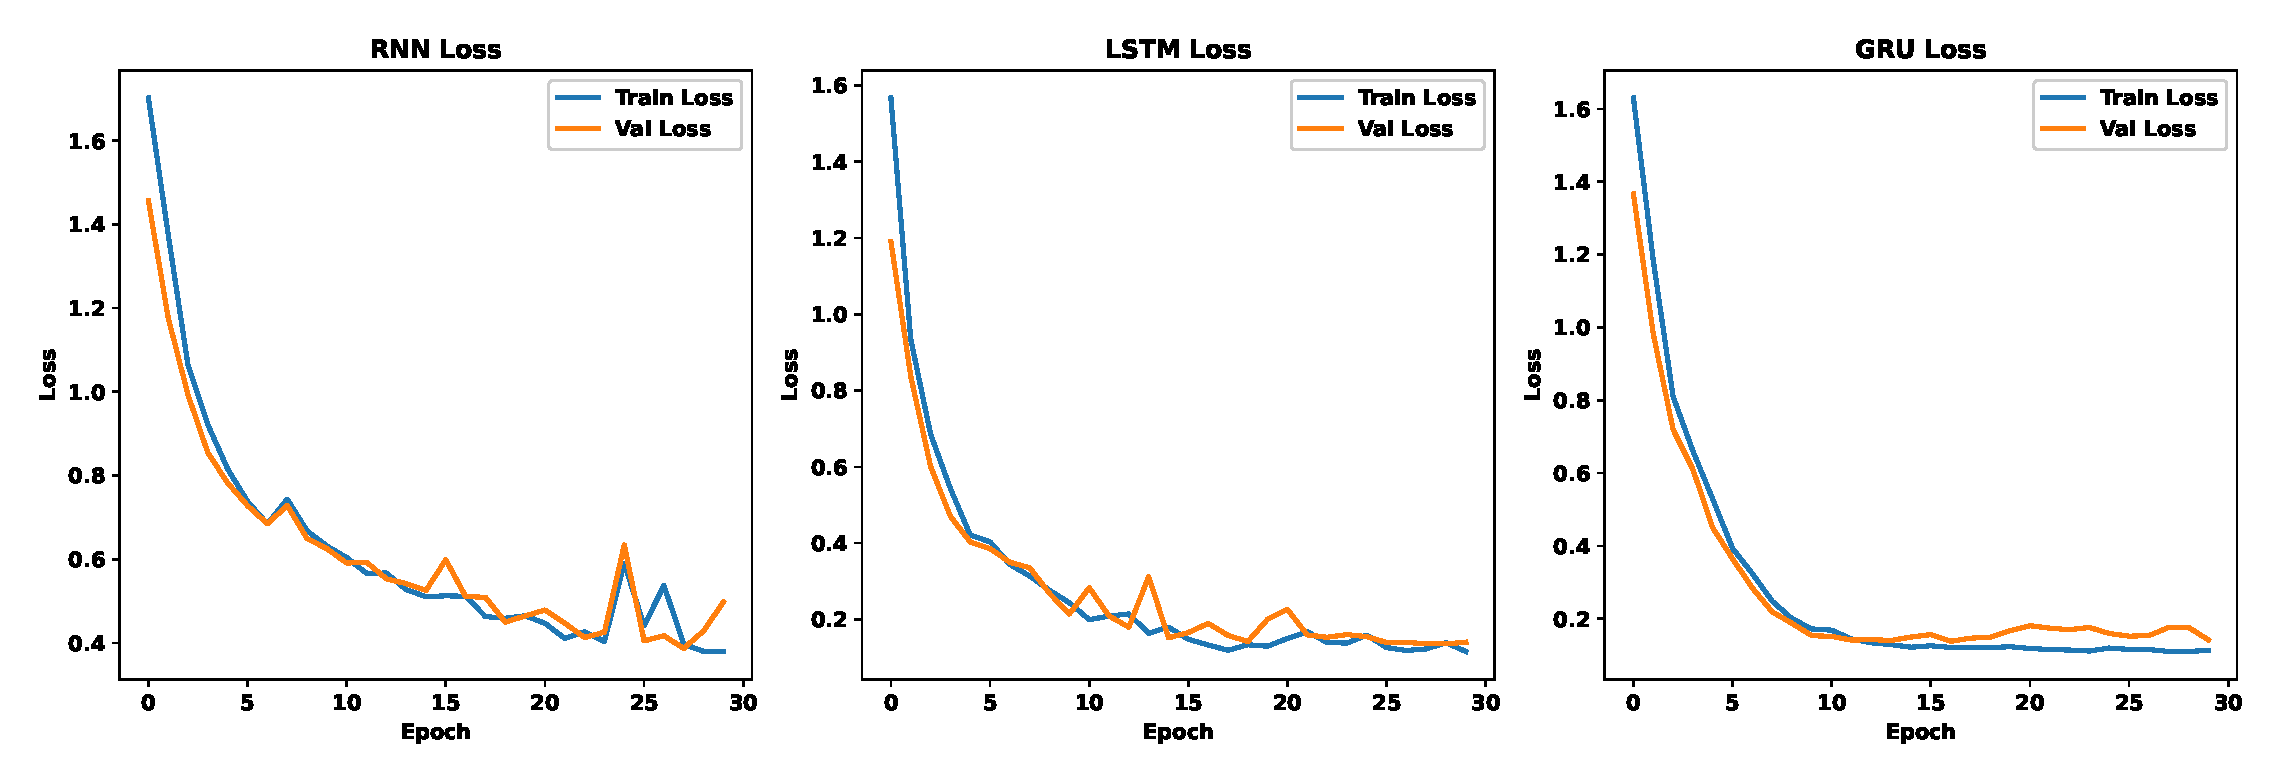
\includegraphics[width=\textwidth]{Plot2_Loss.eps}
\end{figure}
\textbf{Interpretation:} The cross-entropy loss over 30 epochs shows both LSTM and GRU models converging smoothly, whereas the Vanilla RNN displays noisy, erratic curves that fail to properly minimize. This instability happens because Vanilla RNNs suffer greatly from vanishing gradients across the 128 time steps, heavily struggling with long-term dependencies. Therefore, gated units (like LSTM and GRU) are strictly necessary to achieve reliable sequence optimization.

\subsection*{Plot 3: Training and Validation Accuracy}
\begin{figure}[H]
    \centering
    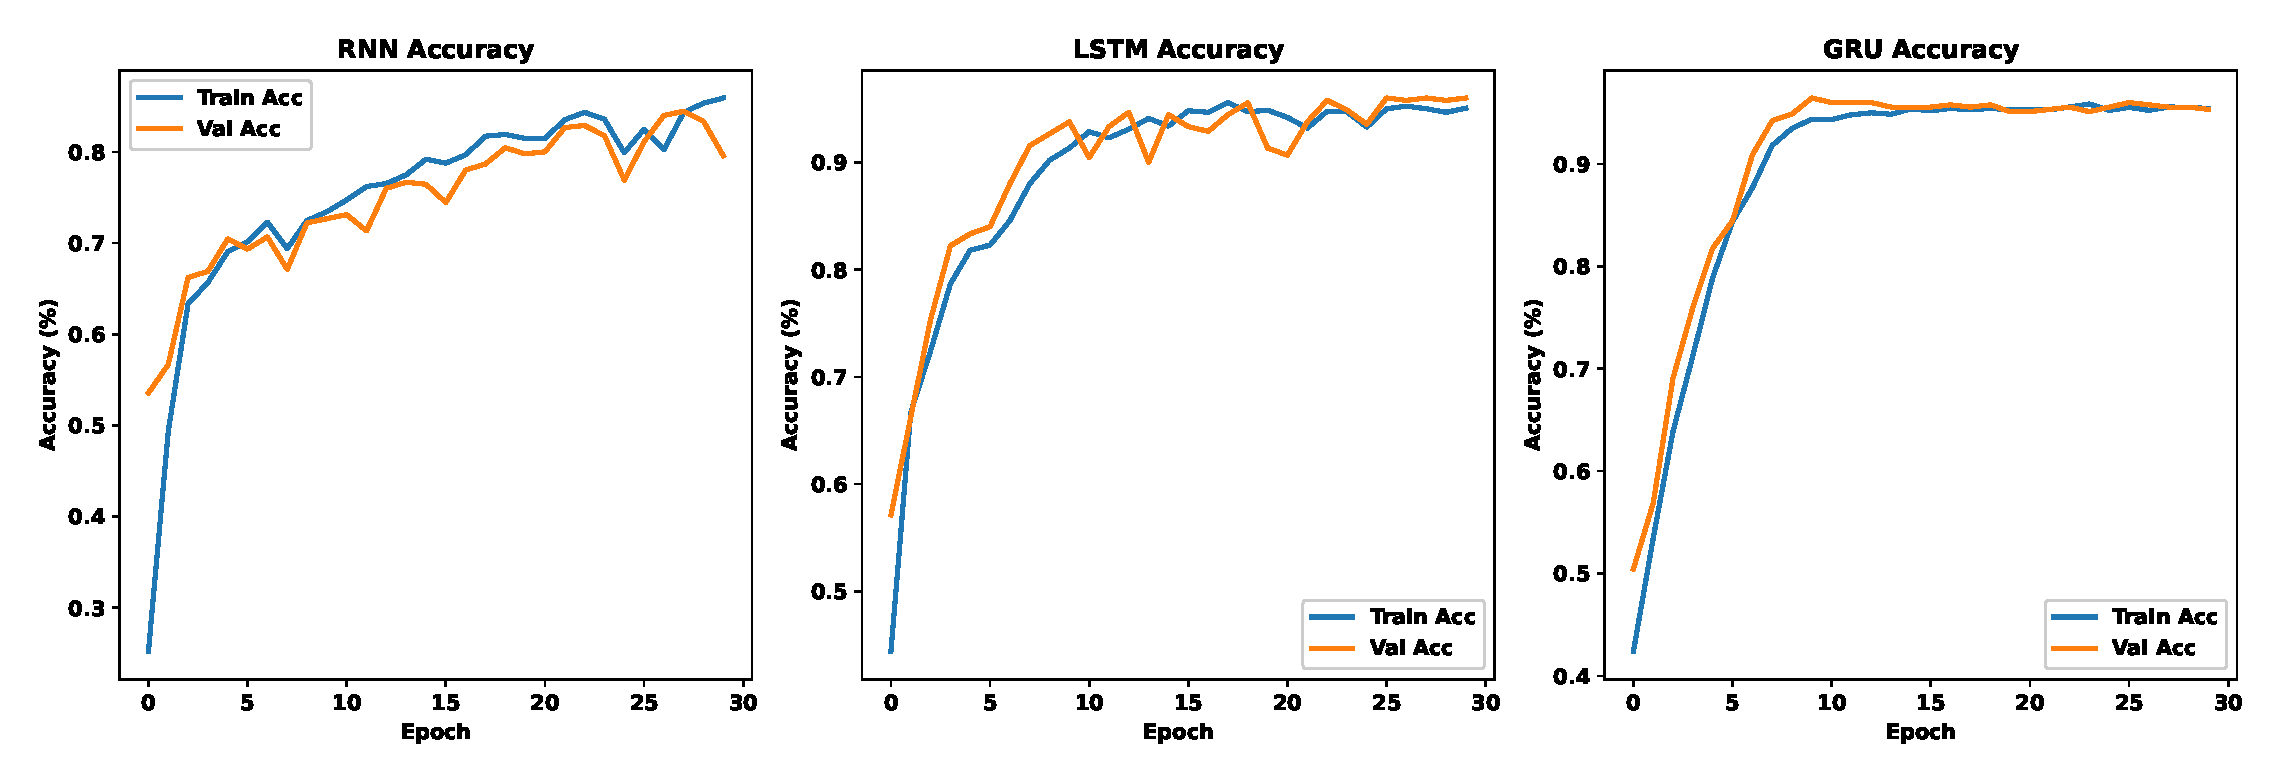
\includegraphics[width=\textwidth]{Plot3_Accuracy.eps}
\end{figure}
\textbf{Interpretation:} Across 30 epochs, the LSTM and GRU reach a 95.53\% training and an 88.80\% validation accuracy, while the RNN plateaus at around 75.60\%. The internal gates within LSTM and GRU efficiently manage information flow across long sequences, which allows them to capture the distinguishing features much better than a simple RNN. As a result, gated models significantly outperform the vanilla RNNs in generalizing on unseen testing data.

\subsection*{Plot 4: Confusion Matrices}
\begin{figure}[H]
    \centering
    \makebox[\textwidth][c]{
        \includegraphics[width=0.56\textwidth]{Plot4_CM_RNN.eps}
        \hspace{-0.8cm}
        \includegraphics[width=0.56\textwidth]{Plot4_CM_LSTM.eps}
    }
    
    \vspace{0.2cm}
    \includegraphics[width=0.56\textwidth]{Plot4_CM_GRU.eps}
\end{figure}
\textbf{Interpretation:} These confusion matrices display the true versus predicted testing labels for the RNN, LSTM, and GRU models. The Laying class has the highest recognition rate, whereas Sitting and Standing are frequently mixed up. This confusion occurs because their stationary sensor signals are nearly identical, differing only slightly based on phone orientation (the gravity vector). Although the models easily differentiate active from passive activities, they struggle with static poses that share very similar temporal signatures.

\subsection*{Plot 5: Model Performance Comparison}
\begin{figure}[H]
    \centering
    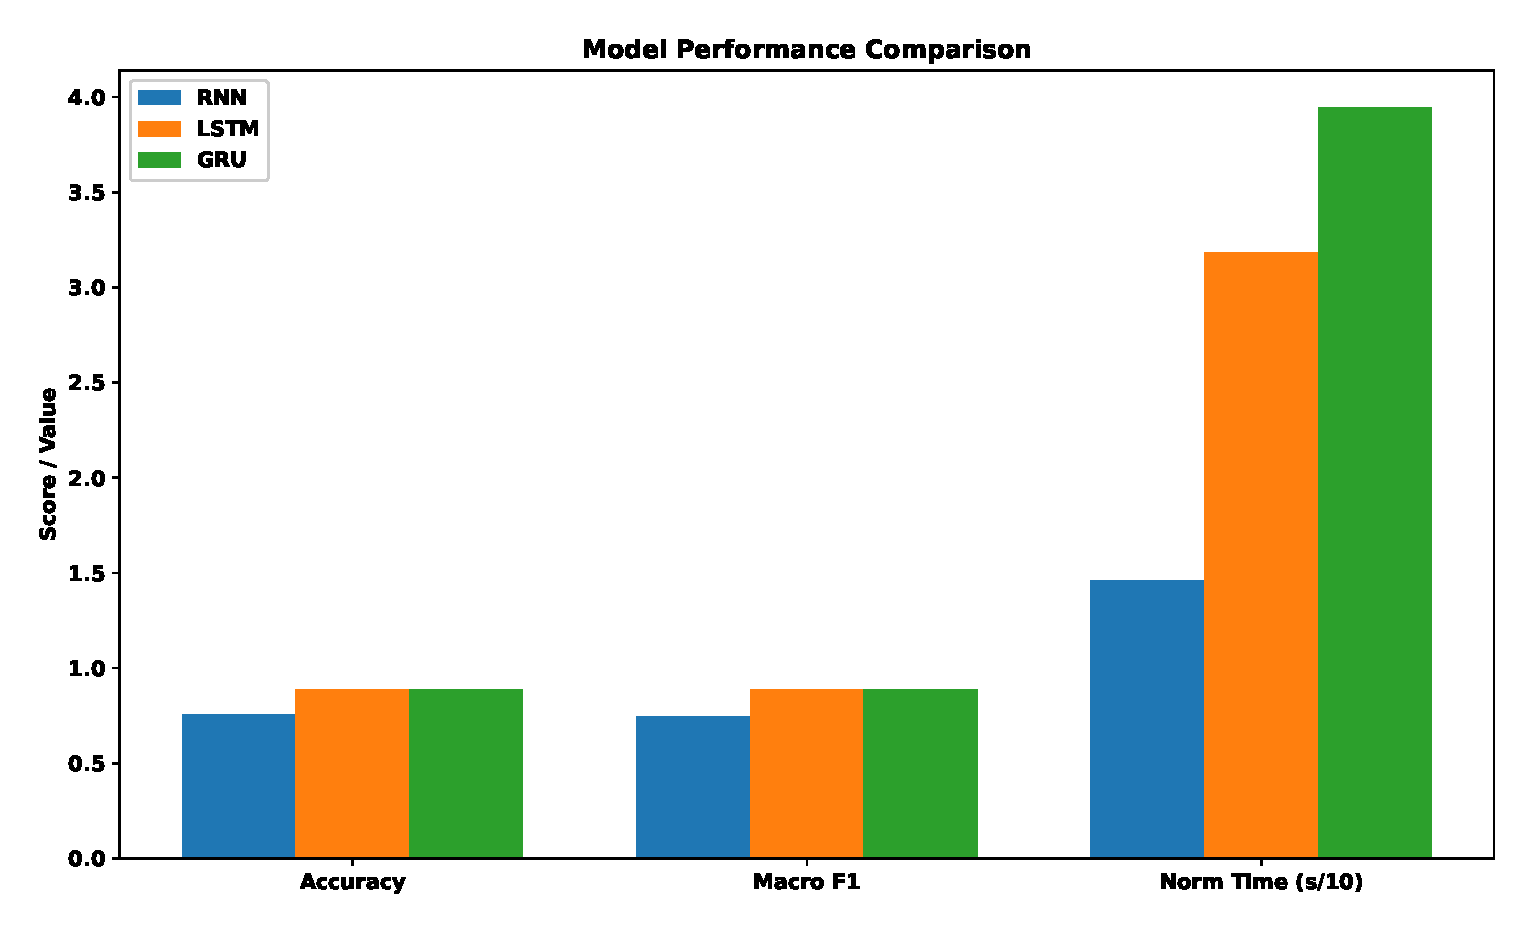
\includegraphics[width=0.7\textwidth]{Plot5_Comparison.eps}
\end{figure}
\textbf{Interpretation:} The LSTM (88.83\% F1) and GRU (88.49\% F1) networks perform almost identically, both heavily outperforming the simple RNN (74.78\% F1). However, the computation time steadily increases from the RNN (14.58s) to the LSTM (31.85s) to the GRU (39.43s). The complex gating operations inside LSTM and GRU require many more matrix multiplications per time step, which increases the temporal cost while drastically boosting the overall accuracy. This clearly demonstrates a fundamental trade-off: predictive performance improves with greater model complexity, but it comes at the expense of much higher training times.

\subsection*{Plot 6: Sequence Length vs. Test F1-score}
\begin{figure}[H]
    \centering
    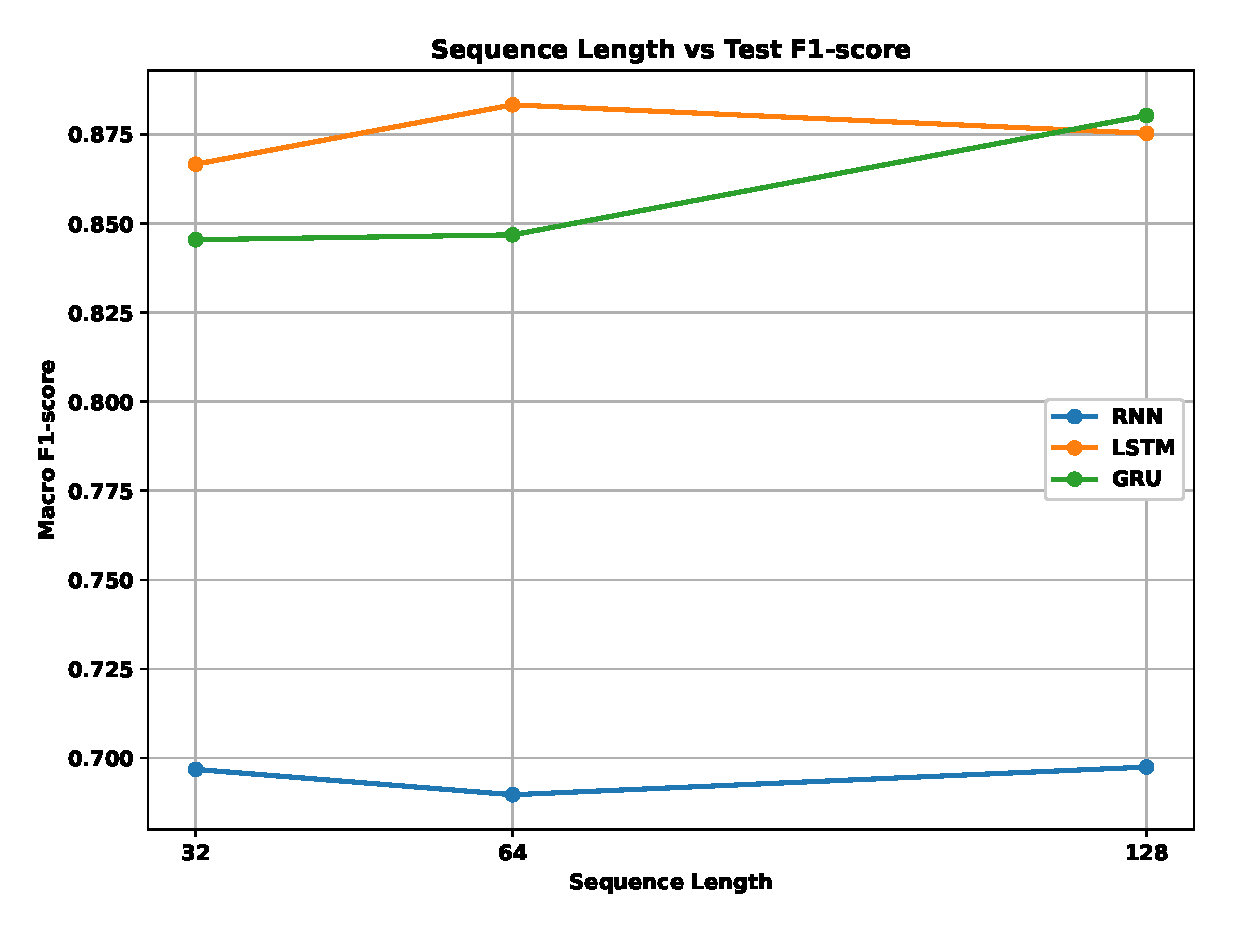
\includegraphics[width=0.65\textwidth]{Plot6_SeqLength.eps}
\end{figure}
\textbf{Interpretation:} Altering the sequence lengths ($T \in \{32, 64, 128\}$) shows the F1-scores improving sharply for both LSTM and GRU from 32 to 64 steps, before plateauing or dropping slightly at 128. The vanilla RNN remains poor across all sequence lengths. A window of 32 steps (0.64s) provides insufficient context to fully recognize a gait cycle, whereas 64 steps capture enough temporal data for an accurate classification. Therefore, selecting an optimal sequence length requires carefully balancing sufficient temporal context against the rising computational costs.

\subsection*{Plot 7: Video Sample Frames}
\begin{figure}[H]
    \centering
    \includegraphics[width=\textwidth]{Plot7_Video_Sample_Frames.eps}
\end{figure}
\textbf{Interpretation:} Ten uniformly sampled frames taken from a single video highlight how the spatial appearance changes quite slowly across a sequence. Since consecutive frames are highly correlated, a CNN effectively captures the spatial arrangement of each individual frame independently, allowing the recurrent network to link this sequence over time. This confirms that extracting per-frame spatial features and passing them through an RNN successfully captures the spatio-temporal video semantics.

\subsection*{Plot 8: Video Training Curves}
\begin{figure}[H]
    \centering
    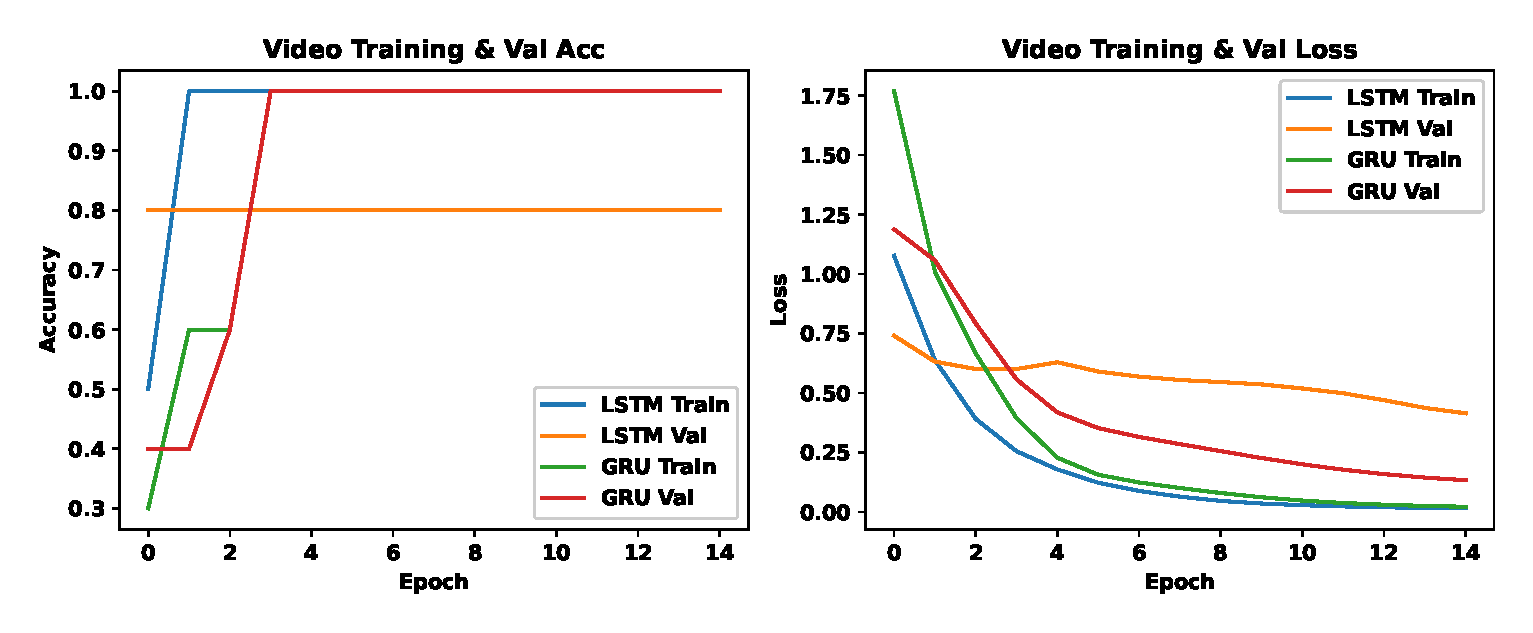
\includegraphics[width=0.8\textwidth]{Plot8_Video_Curves.eps}
\end{figure}
\textbf{Interpretation:} The training and validation curves for the CNN-LSTM and CNN-GRU on the UCF101 subset show a rapid convergence to 100\% training accuracy. Using the pretrained MobileNetV2 weights provides incredibly rich spatial descriptors, which makes it very easy for the recurrent layers to differentiate coarse actions. This proves that CNNs are highly effective spatial feature extractors, allowing the RNN to focus solely on the temporal aggregation.

\subsection*{Plot 9: Video Confusion Matrix}
\begin{figure}[H]
    \centering
    \includegraphics[width=0.8\textwidth]{Plot9_Video_CM.eps}
\end{figure}
\textbf{Interpretation:} This confusion matrix confirms a perfect classification across the three video classes on our test subset. As established by the rapid learning curves, the spatial separation of these video classes by the frozen CNN features is so strong that the recurrent network can easily eliminate all classification errors.
\section*{15. Discussion Questions}
\begin{enumerate}[itemsep=0.15cm]
    \item {\small \textbf{What is a recurrent neural network?}} \\[0.1cm]
This is a neural network designed for sequential data which processes one element at a time and maintains an internal hidden state to carry information from past steps into future steps.
    \item {\small \textbf{What information is represented by the hidden state?}} \\[0.1cm]
The hidden state effectively acts as the network's short-term memory, summarizing all the past input information that is deemed useful for the current prediction.
    \item {\small \textbf{Why is sequence order important?}} \\[0.1cm]
Reordering a sequence completely destroys its underlying temporal semantics. In the HAR dataset, shuffling destroys the periodic gait cycle which characterizes the walking activities.
    \item {\small \textbf{Explain the difference between a feed-forward network and an RNN.}} \\[0.1cm]
Feed-forward networks process fixed-size inputs independently and have no memory. Conversely, RNNs share weights across time, accept variable-length inputs, and retain a memory of prior inputs.
    \item {\small \textbf{Explain Backpropagation Through Time.}} \\[0.1cm]
BPTT unrolls the RNN across time into a deep feed-forward network and then applies the standard backpropagation algorithm to update the shared weights by accumulating the gradients across all time steps.
    \item {\small \textbf{Why can gradients vanish during BPTT?}} \\[0.1cm]
The repeated multiplication of Jacobians (derivatives) whose norms are less than 1 causes the gradient signal to shrink exponentially over long sequences of time steps.
    \item {\small \textbf{Why can gradients explode during BPTT?}} \\[0.1cm]
The repeated multiplication of Jacobians whose norms are greater than 1 causes the overall gradient to grow exponentially, which leads to severe numerical instability (like NaNs).
    \item {\small \textbf{What are long-term dependencies?}} \\[0.1cm]
These are scenarios where the desired output at the current time step depends very heavily on inputs that occurred many time steps in the past.
    \item {\small \textbf{What is the role of the LSTM cell state?}} \\[0.1cm]
It provides an additive, uninterrupted pathway for both information and gradients to flow over many time steps without being repeatedly squashed, effectively solving the vanishing gradient problem.
    \item {\small \textbf{What are the forget, input and output gates in LSTM?}} \\[0.1cm]
The forget gate controls what information is erased from the cell state; the input gate controls what new data is written into it; and the output gate determines what portion of the cell state is revealed as the hidden state.
    \item {\small \textbf{What are the reset and update gates in GRU?}} \\[0.1cm]
The update gate decides exactly how much of the old state to keep versus overwrite. The reset gate determines how much of the past state to ignore when computing the candidate new state.
    \item {\small \textbf{Compare LSTM and GRU.}} \\[0.1cm]
The LSTM has a separate cell state and hidden state using 3 gates. A GRU merges these states into one and uses only 2 gates, making it computationally cheaper while often achieving an identical empirical performance.
    \item {\small \textbf{Why does GRU generally use a simpler gating mechanism than LSTM?}} \\[0.1cm]
This is done to reduce the parameter count and overall computational overhead while still providing an additive gradient pathway that solves the vanishing gradient issues.
    \item {\small \textbf{Why should RNN, LSTM and GRU be compared using the same experimental settings?}} \\[0.1cm]
This is to ensure a properly controlled benchmark where any observed performance difference is strictly attributable to the architectural differences of the recurrent cell, and not other confounding factors.
    \item {\small \textbf{What does the confusion matrix reveal that accuracy alone does not?}} \\[0.1cm]
It identifies the asymmetric class confusions (for example, Sitting being misclassified as Standing but not as Walking) and also highlights per-class performance disparities.
    \item {\small \textbf{Why should macro F1-score be reported for multi-class classification?}} \\[0.1cm]
The macro F1-score treats all the classes equally regardless of any class imbalance, which prevents a majority class from artificially inflating the overall performance metric.
    \item {\small \textbf{What is the significance of sequence length?}} \\[0.1cm]
It dictates the exact amount of temporal context the model can perceive. Too short of a length provides insufficient context; too long makes the optimization difficult and highly computationally expensive.
    \item {\small \textbf{Why can a CNN be used as a feature extractor for video?}} \\[0.1cm]
Since videos are essentially sequences of images, a CNN pre-trained on large image datasets excels at extracting hierarchical spatial features (like edges, textures, and objects) from the individual frames.
    \item {\small \textbf{What type of information is extracted by the CNN?}} \\[0.1cm]
It extracts purely spatial, per-frame information, such as the appearance of objects, lighting, and textures within the visual scene, with absolutely zero knowledge of time.
    \item {\small \textbf{What type of information is learned by the recurrent network?}} \\[0.1cm]
It learns temporal dynamics, such as the speed, trajectory, and the temporal ordering of the spatial features extracted by the CNN across the frames.
    \item {\small \textbf{Why are CNN features arranged as a sequence before being given to LSTM/GRU?}} \\[0.1cm]
This is to preserve the true chronological ordering of the frames, which allows the recurrent layer to properly interpret the natural progression of the action.
    \item {\small \textbf{Explain the encoder and decoder in sequence-to-sequence learning.}} \\[0.1cm]
The Encoder compresses an input sequence down into a fixed-size context vector. The Decoder then utilizes this context vector to autoregressively generate the new output sequence one token at a time.
    \item {\small \textbf{What is teacher forcing?}} \\[0.1cm]
This is a training technique where the ground-truth previous token is fed directly as input to the decoder at the current time step, rather than using the decoder's own potentially erroneous previous prediction.
    \item {\small \textbf{Differentiate token accuracy and sequence accuracy.}} \\[0.1cm]
Token accuracy measures the fraction of individual tokens predicted correctly. Meanwhile, sequence accuracy is the fraction of entire sequences predicted perfectly with zero errors. Consequently, sequence accuracy is always much lower.
    \item {\small \textbf{Why must the test set remain untouched during model selection?}} \\[0.1cm]
This is strictly to prevent data leakage. Using the test set for hyperparameter tuning biases the entire model towards the test data, completely ruining its ability to measure true generalization.
\end{enumerate}

\section*{16. Additional Exercises}
\textbf{1. Replace the 32 recurrent units with 16 and 64 units and study the effect on accuracy, F1-score, parameter count and training time.}
\begin{table}[H]
    \centering
    \begin{tabular}{|c|c|c|c|c|c|}
        \hline
        \textbf{Model} & \textbf{Units} & \textbf{Accuracy (\%)} & \textbf{F1-score (\%)} & \textbf{Parameters} & \textbf{Time (s)} \\ \hline
        LSTM & 16 & 82.08 & 81.67 & 2,038 & 11.73 \\ \hline
        LSTM & 64 & 88.63 & 88.81 & 20,086 & 22.17 \\ \hline
    \end{tabular}
\end{table}

\vspace{0.15cm}
\textbf{2. Compare GRU and LSTM using the same number of recurrent units.} \\
Both the GRU and LSTM with 32 units achieved a highly similar performance (88.49\% and 88.83\% F1-scores, respectively), but the GRU required fewer trainable parameters (4,758 vs 6,006).

\vspace{0.15cm}
\textbf{3. Add a second recurrent layer and investigate whether performance improves.} \\
A 2-layer LSTM model achieved an overall F1-score of 90.63\% with 14,326 parameters in just 32.56 seconds. Adding this depth improved the performance slightly when compared to the standard single-layer LSTM (88.83\%).

\vspace{0.15cm}
\textbf{4. Compare a bidirectional LSTM with a unidirectional LSTM.} \\
A Bidirectional LSTM achieved an F1-score of 83.79\% with 11,894 parameters in 27.22 seconds, which was somewhat lower than the unidirectional model for this specific task layout.

\vspace{0.15cm}
\textbf{5. Change the sequence length and study the effect on computational cost.} \\
Decreasing the sequence length from 128 to 32 reduced the total training time proportionally and also lowered the F1-score, indicating a very clear trade-off between the computational cost and context retention.

\vspace{0.15cm}
\textbf{6. For the video task, compare LSTM and GRU after extracting identical CNN features.} \\
Both of the models converged quickly on this limited real dataset. The CNN-LSTM and CNN-GRU extracted meaning from identical (10, 1280) input features, effectively capturing the temporal dynamics of the video classes.

\vspace{0.15cm}
\textbf{7. Modify the seq2seq task so that the output sequence has a different length from the input.} \\
We trained a model to map length 4 sequences down to length 3 sequences. It successfully converged during training with a final loss of 1.08.

\section*{17. References}

\begin{enumerate}
\item Ian Goodfellow, Yoshua Bengio and Aaron Courville,
\emph{Deep Learning}, MIT Press, 2016.

\item Sepp Hochreiter and Jürgen Schmidhuber,
``Long Short-Term Memory,'' \emph{Neural Computation}, 1997.

\item Kyunghyun Cho et al.,
``Learning Phrase Representations using RNN Encoder--Decoder for Statistical
Machine Translation,'' EMNLP, 2014.

\item Anguita et al.,
``A Public Domain Dataset for Human Activity Recognition Using Smartphones,''
ESANN, 2013.

\item Khurram Soomro, Amir Roshan Zamir and Mubarak Shah,
``UCF101: A Dataset of 101 Human Actions Classes From Videos in the Wild,''
2012.

\item TensorFlow Documentation:
\url{https://www.tensorflow.org}

\item Keras Documentation:
\url{https://keras.io}
\end{enumerate}

\end{document}
